\chapter{Evaluation and Discussion}
\section{Evaluation}
The following evaluations are done according to the provided Gold Standard. In order to evaluate we considered percentage of precision versus recall for each case, then we calculated interpolated precision for four recall level of  25\% 50\%, 75\% and 100\%, and at the end we calculated average value of each level.

\begin{figure}[h]
\caption{Evaluation of our algorithm using the Gold Std shown in a table.}
\centering
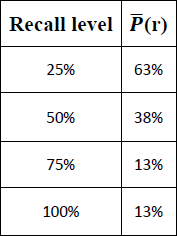
\includegraphics{evaluation_and_discussion/EvalGroup4.png}
\end{figure}

\begin{figure}[h]
\caption{Evaluation of our algorithm using the Gold Std shown in a graph}
\centering
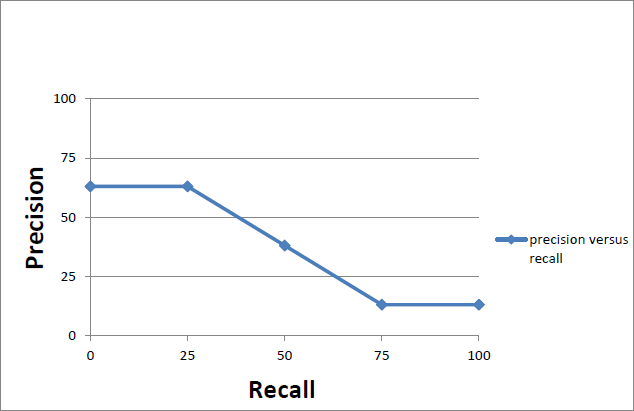
\includegraphics[scale=0.75]{evaluation_and_discussion/EvalGroup4Graph.png}
\end{figure}

\begin{figure}[h]
\caption{Evaluation compared to other groups.}
\centering
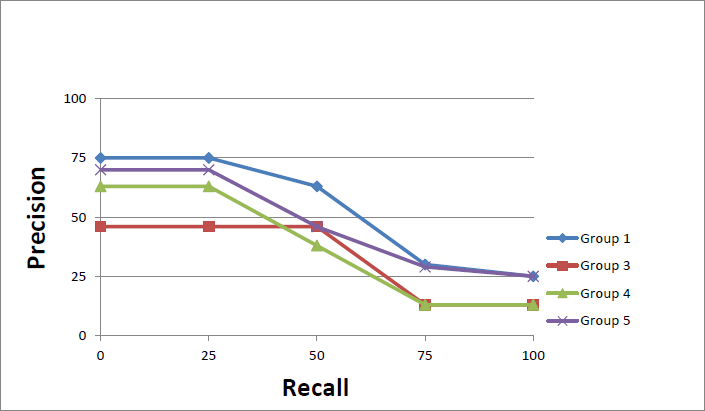
\includegraphics[scale=0.75]{evaluation_and_discussion/TotalEval.png}
\end{figure}

In our algorithm we only considered sub chapters that had their own html-file as separate entities.Therefore, many of the sub chapters in the gold standard did not show up as separate hits in our ranking. This caused that we do not have a relatively good document retrieval. Our precision was not too accurate either, especially for cases like 6, 7, and 8. That relevant documents are in sub chapters is obvious in both the table and graph of precision versus recall.

Search in cases 6 and 8 had a gold standard chapter as the top hit. Exceptions was case 5, which had no relevant chapters, and case 7 with gold chapters on 2. and 4. place. All gold standard chapters can be found via the top 4 hits of our respective case search results.